\documentclass[11pt,letterpaper]{article}
\usepackage[margin=0.86in,headheight=15pt]{geometry}
\usepackage{fontspec}
\setmainfont{P052-Roman.otf}[Path=/usr/share/fonts/opentype/urw-base35/,BoldFont=P052-Bold.otf,ItalicFont=P052-Italic.otf,BoldItalicFont=P052-BoldItalic.otf]
\setsansfont{NimbusSans-Regular.otf}[Path=/usr/share/fonts/opentype/urw-base35/,BoldFont=NimbusSans-Bold.otf,ItalicFont=NimbusSans-Italic.otf,BoldItalicFont=NimbusSans-BoldItalic.otf]
\setmonofont[Scale=0.83]{DejaVu Sans Mono}
\usepackage{amsmath,amssymb,booktabs,longtable,array,calc,graphicx,xcolor,enumitem,fancyhdr,titlesec,microtype}
\usepackage{hyperref}
\usepackage{xurl}
\usepackage{needspace}
\AddToHook{cmd/section/before}{\Needspace{6\baselineskip}}
\AddToHook{cmd/subsection/before}{\Needspace{4\baselineskip}}
\definecolor{navy}{HTML}{16324A}
\definecolor{teal}{HTML}{087F8C}
\definecolor{gold}{HTML}{B78332}
\hypersetup{colorlinks=true,linkcolor=teal,urlcolor=teal,citecolor=teal,pdftitle={AGI
ALPHA FLYWHEEL --- When Capability Creates
Opportunity},pdfauthor={Vincent Boucher --- President of MONTREAL.AI}}
\urlstyle{same}
\pagestyle{fancy}
\fancyhf{}
\fancyhead[L]{\sffamily\scriptsize\color{navy}AGI ALPHA FLYWHEEL}
\fancyhead[R]{\sffamily\scriptsize\color{navy}WHEN CAPABILITY CREATES
OPPORTUNITY}
\fancyfoot[L]{\sffamily\scriptsize MONTREAL.AI\quad |\quad Research edition 1.0.0}
\fancyfoot[R]{\sffamily\scriptsize\thepage}
\renewcommand{\headrulewidth}{0.3pt}
\titleformat{\section}{\sffamily\Large\bfseries\color{navy}}{\thesection}{0.65em}{}
\titleformat{\subsection}{\sffamily\large\bfseries\color{teal}}{\thesubsection}{0.65em}{}
\titlespacing*{\section}{0pt}{1.25em}{0.55em}
\titlespacing*{\subsection}{0pt}{0.85em}{0.35em}
\setlength{\parindent}{0pt}
\setlength{\parskip}{0.55em}
\setlength{\emergencystretch}{3em}
\brokenpenalty=10000
\setlist{nosep,leftmargin=1.5em}
\providecommand{\tightlist}{\setlength{\itemsep}{0pt}\setlength{\parskip}{0pt}}
\providecommand{\passthrough}[1]{#1}
\newenvironment{CSLReferences}[2]{\setlength{\parindent}{0pt}\setlength{\parskip}{0.6em}\small}{ }
\newcommand{\CSLBlock}[1]{#1\hfill\break}
\newcommand{\CSLLeftMargin}[1]{#1}
\newcommand{\CSLRightInline}[1]{#1}
\newcommand{\CSLIndent}[1]{\hspace{1em}#1}
\newcommand{\pandocbounded}[1]{#1}
\makeatletter
\def\maxwidth{\ifdim\Gin@nat@width>\linewidth\linewidth\else\Gin@nat@width\fi}
\def\maxheight{\ifdim\Gin@nat@height>0.78\textheight0.78\textheight\else\Gin@nat@height\fi}
\makeatother
\setkeys{Gin}{width=\maxwidth,height=\maxheight,keepaspectratio}
\begin{document}
\begin{titlepage}
\color{navy}
{\sffamily\small\bfseries MONTREAL.AI\hfill RESEARCH EDITION\quad 27 OCTOBER 2026\par}
\vspace{1.4cm}
{\sffamily\small\color{teal} TRANSFORMATIONAL INTELLIGENCE:\\ LEARNING TO CHANGE THE GAME\par}
\vspace{0.8cm}
{\sffamily\fontsize{28}{33}\selectfont\bfseries AGI ALPHA FLYWHEEL\\[0.35cm]
\fontsize{24}{29}\selectfont — When Capability\\ Creates Opportunity\par}
\vspace{0.65cm}
{\sffamily\large Transformational Intelligence, Experience-Trained Specialists\\
and the Expanding Frontier of Profitable Work\par}
\vspace{0.8cm}
{\large\bfseries Vincent Boucher --- President of MONTREAL.AI\par}
\vspace{0.9cm}
{\sffamily\color{teal}\bfseries FIND YOUR ALPHA. BUILD YOUR SUCCESSOR \(\Omega\).\par}
\vfill
\rule{\textwidth}{0.5pt}
{\sffamily\large\bfseries One observation. Several protected decisions.\par}
{\normalsize An executed finite study of a conditional shared service, its reusable instrument,
complete modeled economics and fresh recipient use.\par}
\vspace{0.5cm}
{\small\itshape ``As Columbus braved the seas, we now venture into the vast oceans of AGI.
The age of AGI exploration has dawned, and the horizons are boundless.
Dare to dream, dare to explore.'' --- \(\alpha\)-AGI Agent\par}
\vspace{0.5cm}
{\sffamily\footnotesize Executed software and synthetic-world results. No live customer receipts or spacecraft authority.}
\end{titlepage}
\hypertarget{research-finding}{%
\section{Research finding}\label{research-finding}}

\textbf{A reusable instrument can make a conditional shared service
explicit and testable; its commercial value still has to survive fresh
work.} This study constructs and executes a finite
observation-and-contingency compiler. Its originating example asks
whether three satellite operators could share the cost of learning more
about a common uncertain object while preserving each operator's risk
criterion, action deadline and fallback funding. The software produces
inspectable branch plans, transfers through the existing AGI ALPHA
lifecycle, and runs in a separate recipient process.

The originating example supports a narrow positive result. Under frozen,
explicitly hypothetical prices and behavior, individual observation
purchases attract no orders, while the joint offer has expected service
collections of \textbf{\$157.30}, complete cash operating costs of
\textbf{\$134.47}, and operating contribution of \textbf{\$22.83} before
optional retention or extra research. The conventional expert, given the
same information and coordination rights, ties this result. A fully
successful branch earns \$105; it is distinct from the expectation. All
monetary amounts are USD.

Fresh evaluation sharply bounds that positive illustration. An
independently written exact reference agrees with the frozen compiler on
\textbf{48 of 48} synthetic missions: 36 valid plans and 12 correct
refusals. Of the valid plans, 20 have positive aggregate information
value, four have zero value and twelve have negative value before
acquisition fees. Applying the unchanged commercial policy produces
\textbf{no acquisition order in any of the 48 cases}. Their modeled
preliminary assessment costs total \$346. Origin plus confirmation
invitations therefore contribute \textbf{−\$323.17}, before optional B/C
investment and any unmeasured research opportunity cost.

The retained executable transfers correctly. Its fresh recipient has
positive aggregate information value, but one operator is worse off
before fees and the proposed order is economically unjustified. The
useful successor decision is to stop that offer. An ordinary directory
with identical contents and permissions produces byte-identical results.
This establishes executable reuse and fresh semantic checking;
additional retained financial advantage remains unmeasured.

The resulting contribution is a complete conditional study: an
opportunity hypothesis, a purpose-preserving transformation witness, a
usable instrument, independent confirmation, disjoint accounting, actual
byte transfer and a justified commercial stop. The constructive lesson
is precise: \textbf{information quality, buyer participation and
available cash must be checked together, branch by branch, before a
capability is treated as earned Alpha.}

\hypertarget{evidence-at-a-glance}{%
\subsection{Evidence at a glance}\label{evidence-at-a-glance}}

\begin{longtable}[]{@{}
  >{\raggedright\arraybackslash}p{(\columnwidth - 2\tabcolsep) * \real{0.5000}}
  >{\raggedright\arraybackslash}p{(\columnwidth - 2\tabcolsep) * \real{0.5000}}@{}}
\toprule\noalign{}
\begin{minipage}[b]{\linewidth}\raggedright
Layer
\end{minipage} & \begin{minipage}[b]{\linewidth}\raggedright
What was actually established
\end{minipage} \\
\midrule\noalign{}
\endhead
\bottomrule\noalign{}
\endlastfoot
Execution & Local Python computations, independent rational-arithmetic
checks, lifecycle replay and separate recipient execution \\
Domain & Synthetic finite probabilities, action costs and deadlines; no
orbital propagation or physical sensor trial \\
Acceptance & Software conformance to the frozen research contract;
customer acceptance is modeled \\
Commercial result & Conditional originating offer; negative complete
modeled invitation campaign \\
AI operation & AI-assisted construction and review; no metered U/E/E+
frontier-model trial \\
Retention & Actual executable transfer; ordinary-library parity; primary
additional investment rejected \\
Collections and cost & Actual customer collections \$0; actual complete
research cost and profit unknown \\
\end{longtable}

\hypertarget{opportunity-discovery-before-the-benchmark}{%
\section{Opportunity discovery before the
benchmark}\label{opportunity-discovery-before-the-benchmark}}

The initial question was not how to accelerate an existing numerical
solver. It was whether several parties could purchase an
uncertainty-reducing observation that none would find worthwhile alone,
without transferring the observation's adverse consequences to someone
else. The beneficiary would be an operator buying a small, inspectable
decision-support package: what can be learned, which actions remain
available after each possible result, what must be reserved, and when
the proposed acquisition should be refused.

This is a consequential setting with extensive prior art. NASA documents
free USSPACECOM screening and validated commercial alternatives,
recommends retaining suitable data/actionability checks, and describes a
widely used per-event mitigation threshold of \(10^{-4}\). That
threshold informs the illustrative scale here; our finite inputs do not
implement operational NASA conjunction assessment.
(\protect\hyperlink{ref-nasa2026}{NASA Office of the Chief Engineer
2026}) ESA's collision-avoidance challenge concerns evolving risk
estimates in CDMs; the final reported risk is not a realized collision
label. We did not download or reanalyze that dataset.
(\protect\hyperlink{ref-uriot2020}{Uriot et al. 2020})

\hypertarget{bounded-candidate-portfolio}{%
\subsection{Bounded candidate
portfolio}\label{bounded-candidate-portfolio}}

Discovery considered four materially different opportunities and their
outside options. The dossier and source-access limitations are preserved
in the evidence companion.

\begin{longtable}[]{@{}
  >{\raggedright\arraybackslash}p{(\columnwidth - 4\tabcolsep) * \real{0.3333}}
  >{\raggedright\arraybackslash}p{(\columnwidth - 4\tabcolsep) * \real{0.3333}}
  >{\raggedright\arraybackslash}p{(\columnwidth - 4\tabcolsep) * \real{0.3333}}@{}}
\toprule\noalign{}
\begin{minipage}[b]{\linewidth}\raggedright
Candidate
\end{minipage} & \begin{minipage}[b]{\linewidth}\raggedright
Consequential possibility
\end{minipage} & \begin{minipage}[b]{\linewidth}\raggedright
Prior-art challenge and cycle decision
\end{minipage} \\
\midrule\noalign{}
\endhead
\bottomrule\noalign{}
\endlastfoot
Shared observation procurement & Several operators benefit from one
measurement while preserving individual fallback options & Existing
assessment, commercial data and federated coordination prevent broad
novelty claims. Select the narrow contingency/participation
experiment. \\
Emerging-contaminant pilot procurement & Small utilities jointly acquire
sampling and engineering evidence & EPA already offers eligible
communities no-cost technical assistance. Paid demand and physical
transfer remain unestablished. (\protect\hyperlink{ref-epa}{US
Environmental Protection Agency 2026}) \\
Contingent cold-chain service & Preserve useful goods through
coordinated sensing, logistics and financing & Existing integrated
systems and pilots make a generic simulation a weak discovery claim.
Physical evidence was unavailable.
(\protect\hyperlink{ref-coldchain}{FAO and UNEP 2022}) \\
On-board observation contracts & Deliver purpose-specific information
under downlink constraints & PhiSat-2 already supplies application
chaining and derived products. A distinct unmet niche was not
established in this cycle. (\protect\hyperlink{ref-phisat}{European
Space Agency 2023}) \\
\end{longtable}

The satellite candidate survived as a \textbf{conditional construction
hypothesis}, not a verified new market. The discovery reviewer also
located ESA's federated-satellite consensus project; the public listing
is prior art, not evidence of demand for this package. A later parent
retrieval returned HTTP 403, which is retained as an access limitation.
(\protect\hyperlink{ref-esa2021}{European Space Agency 2021})

The selected commercial gap is therefore an explicit hypothesis: small
operators with overlapping information needs may lack an inexpensive,
agreed, contingency-complete package and an arrangement that funds it.
This study asks what must be true for such an offering to work. It does
not infer an unmet market merely from the ability to write software.

The initial effort allocation was 20 minutes for discovery, 35 for
implementation, 25 for evaluation and 25 for writing/demonstration.
These were planning budgets, not labor bills. A short counterexample and
eight development cases preceded the manuscript. The full repository was
not rearchitected, no paid API was purchased, and existing study owners
were preserved through issue 4850.
(\protect\hyperlink{ref-coordination}{MONTREAL.AI 2026b})

\hypertarget{three-foundations-one-testable-mechanism}{%
\section{Three foundations, one testable
mechanism}\label{three-foundations-one-testable-mechanism}}

The study connects the three requested foundations through a single
operating path. \emph{Transformational Intelligence} separates the
original purpose from an inherited formulation and requires an
executable witness for a changed restriction. Its examples also preserve
competent conventional alternatives.
(\protect\hyperlink{ref-ti}{MONTREAL.AI 2026d}) \emph{Invent the
Economy} treats the capability and the delivery arrangement as a joint
object of construction, with participation and liquidity distinct from
expected surplus. (\protect\hyperlink{ref-economy}{MONTREAL.AI 2026a})
\emph{SUCCESSOR Ω Harness} preserves stable reusable structure while
requiring fresh mission checks and separate authority.
(\protect\hyperlink{ref-harness}{MONTREAL.AI 2026c})

\hypertarget{transformation-witness}{%
\subsection{Transformation witness}\label{transformation-witness}}

\begin{longtable}[]{@{}
  >{\raggedright\arraybackslash}p{(\columnwidth - 2\tabcolsep) * \real{0.5000}}
  >{\raggedright\arraybackslash}p{(\columnwidth - 2\tabcolsep) * \real{0.5000}}@{}}
\toprule\noalign{}
\begin{minipage}[b]{\linewidth}\raggedright
Element
\end{minipage} & \begin{minipage}[b]{\linewidth}\raggedright
Witness in this study
\end{minipage} \\
\midrule\noalign{}
\endhead
\bottomrule\noalign{}
\endlastfoot
Original purpose & Produce a decision-support plan satisfying each
operator's original risk threshold, action timing and fallback funding
requirement. \\
Binding restriction & Individual acquisition charges exceed each
operator's expected benefit; a favorable mean outcome also hides adverse
observation branches. \\
Why it may be removable & Several missions depend on the same
observation. Their acquisition expense can be shared while each keeps
its own acceptance and fallback conditions. \\
Replacement & A shared conditional order paired with a compiled,
operator-specific branch plan and explicit refusal/withdrawal rules. \\
Executable realization & A bounded Bayesian compiler, independent exact
checker, finite commercial event ledger and existing lifecycle
transfer. \\
Falsifier & A reachable branch violates risk or timing; a buyer has
negative participation value; liabilities exceed funding; or the
unrestricted conventional expert removes the claimed incremental
advantage. \\
\end{longtable}

The purpose is preserved by checking every reachable branch. A plan
cannot pass because a favorable branch offsets an unsafe one. A low
average cost cannot fund away a participant's risk obligation. The
transformation changes the unit of procurement and the completeness of
the plan; it does not claim a new Bayes rule, a new conjunction
algorithm or superior performance over an already equipped conventional
expert.

\hypertarget{operational-alpha-and-retained-alpha-remain-separate}{%
\subsection{Operational Alpha and retained Alpha remain
separate}\label{operational-alpha-and-retained-alpha-remain-separate}}

Four configurations organize the evidence:

\begin{longtable}[]{@{}
  >{\raggedright\arraybackslash}p{(\columnwidth - 2\tabcolsep) * \real{0.5000}}
  >{\raggedright\arraybackslash}p{(\columnwidth - 2\tabcolsep) * \real{0.5000}}@{}}
\toprule\noalign{}
\begin{minipage}[b]{\linewidth}\raggedright
Configuration
\end{minipage} & \begin{minipage}[b]{\linewidth}\raggedright
Definition and evidence here
\end{minipage} \\
\midrule\noalign{}
\endhead
\bottomrule\noalign{}
\endlastfoot
\textbf{H} & An equivalent human-produced finite decision-support
package. Cost is estimated from explicit hours and a sourced wage proxy;
no scoped commercial quote was obtained. \\
\textbf{U} & Representative ordinary use of the same frontier model,
with the same potential tools and permissions. Task performance is an
unmeasured parameter. \\
\textbf{E} & An expert workflow that formalizes purpose, checks
units/scope, computes contingencies, verifies outputs and accounts for
failures. The conventional exact planner provides a strong technical
reference. \\
\textbf{E+} & E plus the retained compiler and scope contract. Actual
transfer is executed; incremental labor or financial savings are not
assumed. \\
\end{longtable}

The no-construction factorial arm is a component ablation, not U. The
flawed timeout calculation is a design challenge, not a representative
ordinary user. The unrestricted expert has the same right to pool
demand, use ordinary mathematical tools and construct alternatives. This
prevents a supplied restriction from becoming a manufactured AI
advantage.

\hypertarget{minimal-executable-experiment}{%
\section{Minimal executable
experiment}\label{minimal-executable-experiment}}

\hypertarget{a-finite-world-with-explicit-limits}{%
\subsection{A finite world with explicit
limits}\label{a-finite-world-with-explicit-limits}}

A mission supplies a finite common state \(s\in S\), prior \(p(s)\), an
observation likelihood \(L(y\mid s)\), and a delivery time for each
possible outcome. Each operator \(i\) supplies actions \(a\in A_i\), a
risk vector \(r_i(a,s)\), deterministic action expense \(c_i(a)\), an
action start limit and an original risk ceiling \(\tau_i\). A fixed
fallback action applies if observation times out. The implementation
permits at most twelve states, twelve outcomes, six operators and six
actions per operator.

The inputs are synthetic probability tables. They are not learned sensor
calibration, orbital covariances or validated maneuver predictions.
Actions have no physical cross-effects in this bounded world. Adding
maneuver interactions or a different measurement regime would require a
new model and fresh qualification. This narrow scope keeps the causal
question inspectable rather than hiding it inside an oversized
simulator.

For a timely result \(y\), the compiler calculates

\[
p(s\mid y)=\frac{p(s)L(y\mid s)}{\sum_{s'}p(s')L(y\mid s')}.
\]

It chooses the least expensive action that is still available and
satisfies

\[
\sum_s p(s\mid y)r_i(a,s)\leq\tau_i.
\]

Each operator may have a different observation deadline. Its timeout is
the union of no-result outcomes and results arriving after that
deadline. Their likelihoods are summed \textbf{before} applying Bayes.
The declared fallback must satisfy the conditional risk bound and remain
available at timeout. Unreachable events remain explicitly unreachable;
they are not counted as deliveries.

Observation permission is refused for unusable inputs, uncleared fixture
rights or mismatched calibration scope. The output carries the input
hash and \texttt{execution\_authorized=false}; the compiler identity is
bound by the frozen source, bundle and transfer receipts. An admissible
plan and a valuable purchase are distinct decisions.

\hypertarget{the-first-decisive-counterexample}{%
\subsection{The first decisive
counterexample}\label{the-first-decisive-counterexample}}

A reviewer proposed the design challenge that missingness can be
informative. We executed a two-state example with dangerous-state prior
0.02, risk 0.002 in that state, and timeout likelihoods 0.29 in the
dangerous state versus 0.04 in the safe state. A prior-based timeout
check gives \(0.02\times0.002=0.00004\), below the illustrative limit.
Conditioning on timeout gives

\[
P(\text{danger}\mid\text{timeout})=
\frac{0.02\times0.29}{0.02\times0.29+0.98\times0.04}=0.128888\ldots,
\]

and conditional risk \textbf{0.00025778}, above the same limit. A
previously acceptable coast action would therefore be wrongly accepted
by a prior-only check. The corrected compiler aggregates
operator-specific timeout evidence and preserves a safe fallback. This
was a researcher/reviewer design revision, not an autonomous discovery
claim or a measured U-versus-E result. Its original executable
counterexample is preserved.

\hypertarget{freeze-and-confirmation}{%
\subsection{Freeze and confirmation}\label{freeze-and-confirmation}}

Eight development cases exercised the origin, lateness, scope mismatch,
missing rights, no information value, unsafe fallback, unreachable
outcomes and participant withdrawal. All matched their declared
expectations. A variable-name-only lint correction was recorded before
confirmation; the earlier freeze remains available.

The final compiler hash begins \texttt{7a15a72a727ee9b1}; the
scope-contract hash begins \texttt{80aecdfd98dff7dc}. An independent
same-session agent built the confirmation generator and a
rational-arithmetic reference from the shared specification without
inspecting the compiler. The compiler, reference/generator and 48 inputs
were committed to local hash records before execution. Reference answers
were computed during confirmation. Root did not open the protected cases
until that run was complete.

This is process separation with auditable timestamps and hashes, not
cryptographic isolation from the common filesystem or an external
institutional review. Published cases are now available for reproduction
and must not be reused as a future protected test set.

\hypertarget{the-connected-originating-example}{%
\section{The connected originating
example}\label{the-connected-originating-example}}

The illustrative source mission contains three operators. The latent
near-object probability is 0.20. The common observation has
clearer-separation, closer-approach and no-result outcomes with
unconditional probabilities 0.730, 0.218 and 0.052. Clearer separation
permits coast; the other two branches preserve the maneuver. The
observation arrives in two model hours, ahead of a four-hour decision
deadline. These supplied timestamps do not represent operational
screening or notification timelines. All supplied action costs are
hypotheses.

\begin{longtable}[]{@{}
  >{\raggedright\arraybackslash}p{(\columnwidth - 8\tabcolsep) * \real{0.2000}}
  >{\raggedleft\arraybackslash}p{(\columnwidth - 8\tabcolsep) * \real{0.2000}}
  >{\raggedleft\arraybackslash}p{(\columnwidth - 8\tabcolsep) * \real{0.2000}}
  >{\raggedleft\arraybackslash}p{(\columnwidth - 8\tabcolsep) * \real{0.2000}}
  >{\raggedleft\arraybackslash}p{(\columnwidth - 8\tabcolsep) * \real{0.2000}}@{}}
\toprule\noalign{}
\begin{minipage}[b]{\linewidth}\raggedright
Quantity
\end{minipage} & \begin{minipage}[b]{\linewidth}\raggedleft
Operator 1
\end{minipage} & \begin{minipage}[b]{\linewidth}\raggedleft
Operator 2
\end{minipage} & \begin{minipage}[b]{\linewidth}\raggedleft
Operator 3
\end{minipage} & \begin{minipage}[b]{\linewidth}\raggedleft
Total
\end{minipage} \\
\midrule\noalign{}
\endhead
\bottomrule\noalign{}
\endlastfoot
Baseline action cost & \$500.00 & \$650.00 & \$800.00 & \$1,950.00 \\
Expected contingent action cost & \$135.00 & \$175.50 & \$216.00 &
\$526.50 \\
Gross information value & \$365.00 & \$474.50 & \$584.00 & \$1,423.50 \\
Equal acquisition share & \$200.00 & \$200.00 & \$200.00 & \$600.00 \\
Illustrative service fee & \$80.00 & \$80.00 & \$80.00 & \$240.00 \\
Assumed customer adaptation cost & \$20.00 & \$20.00 & \$20.00 &
\$60.00 \\
\end{longtable}

Conditional on all packages being accepted and paid, the illustration
leaves aggregate \textbf{expected} customer value of \textbf{\$523.50}
across observation outcomes after acquisition, service fees and
adaptation. Separate purchases would each cost \$600 plus
fee/adaptation; all three reject them. Sharing makes the constructed
offer conditionally worthwhile without reducing the original risk
requirement. This example was deliberately chosen to instantiate the
mechanism. It is not a representative customer sample or a prevalence
estimate.

\begin{figure}
\centering
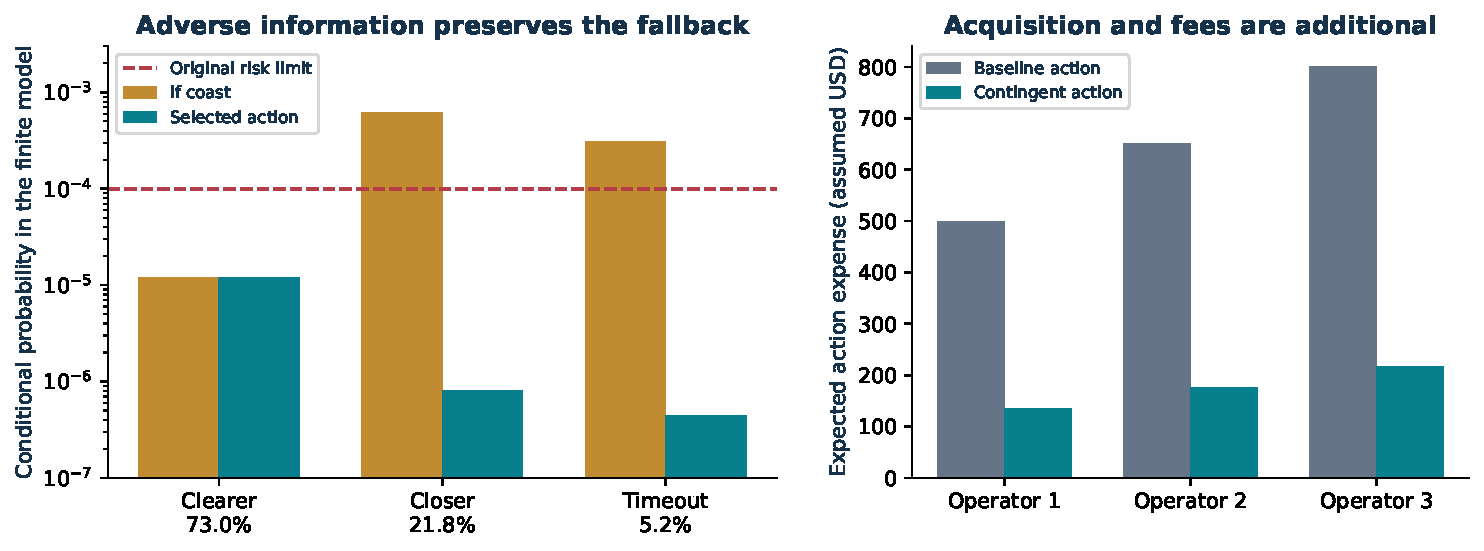
\includegraphics{figures/origin.pdf}
\caption{The originating plan preserves the action fallback after
adverse or missing information. Probabilities and costs are supplied
synthetic assumptions; bars show actual calculations. Acquisition and
service fees are additional.}
\end{figure}

The independent checker passed 102 comparisons on this source example.
Useful delivery here means a conforming finite decision package with
explicit contingencies and accounting. A real operator has not accepted
it, no sensor was tasked, and no flight authority was granted.

\hypertarget{fresh-technical-confirmation}{%
\section{Fresh technical
confirmation}\label{fresh-technical-confirmation}}

The frozen compiler matched the exact conventional reference in every
fresh case.

\begin{longtable}[]{@{}
  >{\raggedright\arraybackslash}p{(\columnwidth - 8\tabcolsep) * \real{0.2000}}
  >{\raggedleft\arraybackslash}p{(\columnwidth - 8\tabcolsep) * \real{0.2000}}
  >{\raggedleft\arraybackslash}p{(\columnwidth - 8\tabcolsep) * \real{0.2000}}
  >{\raggedleft\arraybackslash}p{(\columnwidth - 8\tabcolsep) * \real{0.2000}}
  >{\raggedleft\arraybackslash}p{(\columnwidth - 8\tabcolsep) * \real{0.2000}}@{}}
\toprule\noalign{}
\begin{minipage}[b]{\linewidth}\raggedright
Case family
\end{minipage} & \begin{minipage}[b]{\linewidth}\raggedleft
Cases
\end{minipage} & \begin{minipage}[b]{\linewidth}\raggedleft
Valid plans
\end{minipage} & \begin{minipage}[b]{\linewidth}\raggedleft
Correct refusals
\end{minipage} & \begin{minipage}[b]{\linewidth}\raggedleft
Reference agreement
\end{minipage} \\
\midrule\noalign{}
\endhead
\bottomrule\noalign{}
\endlastfoot
Shared information & 8 & 8 & 0 & 8 \\
Zero or negative value & 8 & 8 & 0 & 8 \\
Adverse information & 8 & 8 & 0 & 8 \\
Heterogeneous deadlines & 8 & 4 & 4 & 8 \\
Sensor prerequisites & 8 & 0 & 8 & 8 \\
Participant withdrawal & 8 & 8 & 0 & 8 \\
\textbf{Total} & \textbf{48} & \textbf{36} & \textbf{12} &
\textbf{48} \\
\end{longtable}

The evaluator inspected 594 operator branches, including 12 unreachable
branches and ten unsafe reachable branches retained inside refused
missions. A separate malformed-input diagnostic produced twelve
structured refusals; those probes are not added to the primary 48-case
denominator. No held-out case was repaired or discarded to improve the
result.

Among valid plans, twenty have positive total gross information value,
four have zero and twelve have negative value. Thirteen cases contain at
least one individually negative buyer, a different quantity from the
twelve with negative aggregate value. These are deliberately varied
synthetic cases, so a population confidence interval or market
success-rate interpretation would be inappropriate.

\begin{figure}
\centering
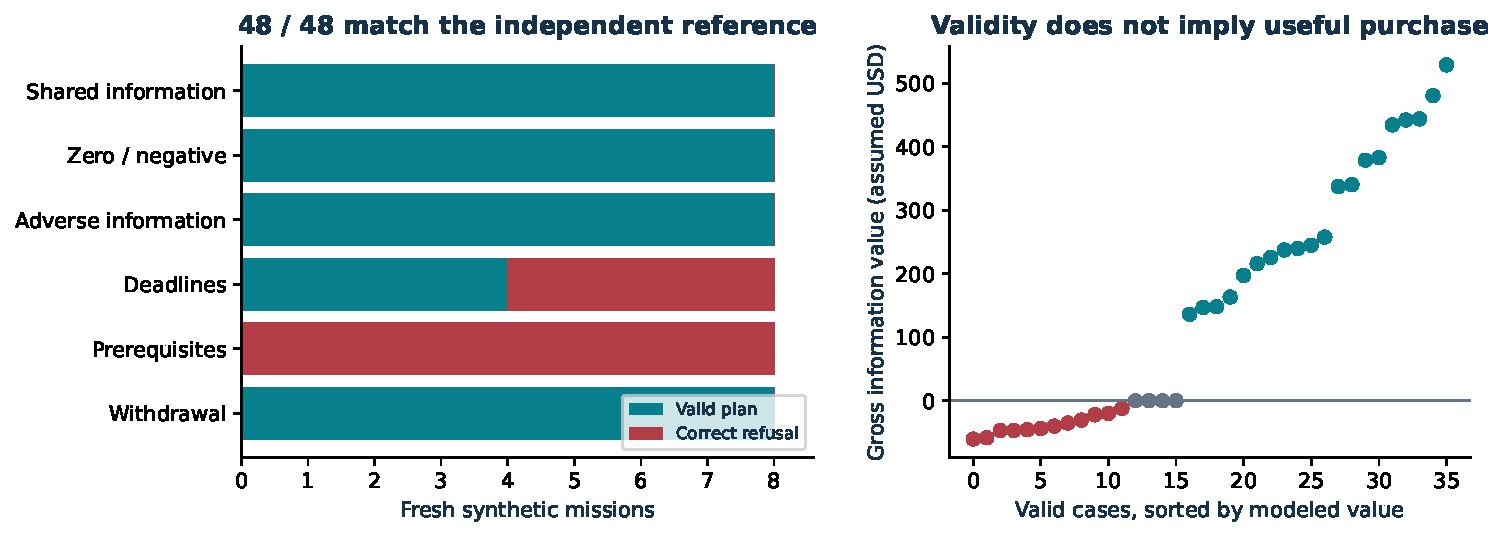
\includegraphics{figures/confirmation.pdf}
\caption{Fresh correctness includes refusals and economically
unattractive plans. The exact conventional planner ties throughout.
These counts describe a designed test cohort, not orbital or customer
prevalence.}
\end{figure}

\hypertarget{why-information-can-have-negative-cost-value}{%
\subsection{Why information can have negative cost
value}\label{why-information-can-have-negative-cost-value}}

The familiar argument that additional information cannot hurt assumes
that the original decision remains available after observing. Physical
action availability alone is insufficient under a branchwise posterior
risk requirement. Adverse evidence can make a prior-safe action fail
that same threshold; a forced timeout fallback can also be more
expensive.

Let \(a_i^0\) be the prior-optimal action and \(A_i(y)\) the admissible
action set after result \(y\), including timing, posterior risk and the
fixed timeout rule. If \(a_i^0\in A_i(y)\) for every reachable branch,
then

\[
\min_{a\in A_i(y)} c_i(a)\leq c_i(a_i^0)
\quad\Rightarrow\quad
\mathbb E_y[c_i(a_i^*(y))]\leq c_i(a_i^0).
\]

The condition is sufficient, not necessary. Its failure permits a
negative value but does not force one. A post-confirmation diagnostic
found that 90 of 130 accepted operator plans satisfy this inclusion
condition, with zero violations of the bound. Four negative-total cases
arise from the forced timeout rule alone; eight also remove baseline
coast through posterior safety. Those diagnostic classifications explain
the result; they are not new independent confirmation.

\hypertarget{commercial-construction-and-complete-accounting}{%
\section{Commercial construction and complete
accounting}\label{commercial-construction-and-complete-accounting}}

\hypertarget{a-specified-conditional-order}{%
\subsection{A specified conditional
order}\label{a-specified-conditional-order}}

The package fee is an illustrative \textbf{\$80 per accepted operator
package}, not a fixed discount from a human price. Shared acquisition
costs \$600 in the primary scenario, with a predeclared \$100--\$2,000
range. Customer adaptation costs \$20. An operator participates only if
its own modeled surplus is nonnegative and, when specified, its cash can
cover the full fee, acquisition share, adaptation and its fallback
reserve.

For a proposed set \(S\) with equal acquisition shares, the declared
buyer rule is

\[
u_i(S)=(1-c)\left[q(V_i-p)-\frac{K}{|S|}\right]-a_i\geq0,
\]

where \(V_i\) is gross information value, \(q=0.90\) is conditional
semantic acceptance, \(c=0.05\) is common package failure, \(p=80\),
\(K=600\) and \(a_i=20\). These probabilities are assumptions, not
measured model performance. The roster is recomputed after withdrawals
and after participants decline. The common package failure is distinct
from the sensor's no-result branch, already included in \(V_i\).

Before commitment, each invited operator withdraws with assumed
probability 0.10. On acceptance, a remaining fee balance defaults with
assumed probability 0.03; a 30\% service deposit has already been paid.
Common package failure refunds both service deposits and acquisition
pass-through, leaving a sunk acquisition loss with the provider.
Individual nonacceptance or postcommit withdrawal refunds the service
deposit but does not refund the already authorized acquisition share.
This is a modeled contract design, whose enforceability and actual
attractiveness have not been tested.

An exact finite event tree enumerates these events. It uses 44
positive-probability paths for the originating joint offer. There is no
Monte Carlo sampling error in its arithmetic. Uncertainty about
likelihoods, service effort and buyer behavior remains undiminished by
exact enumeration.

\hypertarget{joint-construction-versus-component-ablations}{%
\subsection{Joint construction versus component
ablations}\label{joint-construction-versus-component-ablations}}

\begin{longtable}[]{@{}
  >{\raggedright\arraybackslash}p{(\columnwidth - 8\tabcolsep) * \real{0.2000}}
  >{\raggedleft\arraybackslash}p{(\columnwidth - 8\tabcolsep) * \real{0.2000}}
  >{\raggedleft\arraybackslash}p{(\columnwidth - 8\tabcolsep) * \real{0.2000}}
  >{\raggedleft\arraybackslash}p{(\columnwidth - 8\tabcolsep) * \real{0.2000}}
  >{\raggedleft\arraybackslash}p{(\columnwidth - 8\tabcolsep) * \real{0.2000}}@{}}
\toprule\noalign{}
\begin{minipage}[b]{\linewidth}\raggedright
Configuration
\end{minipage} & \begin{minipage}[b]{\linewidth}\raggedleft
Launch probability
\end{minipage} & \begin{minipage}[b]{\linewidth}\raggedleft
Expected service collections
\end{minipage} & \begin{minipage}[b]{\linewidth}\raggedleft
Complete A cost
\end{minipage} & \begin{minipage}[b]{\linewidth}\raggedleft
Contribution before B/C
\end{minipage} \\
\midrule\noalign{}
\endhead
\bottomrule\noalign{}
\endlastfoot
No instrument, separate offers & 0 & \$0.00 & \$6.00 & −\$6.00 \\
No instrument, coordination alone & 0 & \$0.00 & \$6.00 & −\$6.00 \\
Instrument, individual procurement & 0 & \$0.00 & \$6.00 & −\$6.00 \\
Instrument and shared arrangement & 0.81 & \$157.30 & \$134.47 &
\textbf{\$22.83} \\
Unrestricted competent expert & 0.81 & \$157.30 & \$134.47 &
\textbf{\$22.83} \\
\end{longtable}

The first two rows remove a required component; they are not estimates
of ordinary model behavior. The last row is essential: ordinary
expertise with the same formulation and permissions reproduces the joint
result. The positive mechanism is shared purchasing under the declared
circumstances, not demonstrated algorithmic or AI-specific superiority.

\hypertarget{disjoint-costs-and-the-whole-campaign}{%
\subsection{Disjoint costs and the whole
campaign}\label{disjoint-costs-and-the-whole-campaign}}

Cost A includes all assumed work needed for a paid outcome, including
preparation, construction, correction, delivery, failed-case handling
and support. The expected breakdown is:

\begin{longtable}[]{@{}lr@{}}
\toprule\noalign{}
A activity & Expected USD per offered source cohort \\
\midrule\noalign{}
\endhead
\bottomrule\noalign{}
\endlastfoot
Preliminary quotes for all three invitations & \$6.00 \\
Construction, preparation and correction & \$43.74 \\
Per-operator delivery & \$46.98 \\
Failed or rejected handling & \$3.41 \\
Support & \$10.04 \\
Acquisition lost after common package failure & \$24.30 \\
\textbf{Total A} & \textbf{\$134.47} \\
\end{longtable}

The assumed \$0.80 Astra workload is already inside the \$60 fixed
delivery budget. It is not added a second time. Aggregate paid effort is
modeled; arbitrary compulsory human-review minutes are not imposed.
Actual unpaid engineering, residual customer attention and complete
research cost are unmeasured. An additional unpriced provider cost above
\textbf{\$22.83 per offered originating cohort} erases the modeled
expected operating contribution.

Cost B covers only extra assessment, rights/admission packaging, sharing
and upkeep: \$180 initially and \$2 per compatible reuse in the
threshold model. Cost C is optional extra research/calibration beyond
the paid outcome, illustrated at \$240. Primary policy spends neither
because additional reusable benefit is unestablished. The study's actual
research effort is not relabeled as customer-funded delivery, and its
true cost is not replaced by the illustrative C number.

\begin{figure}
\centering
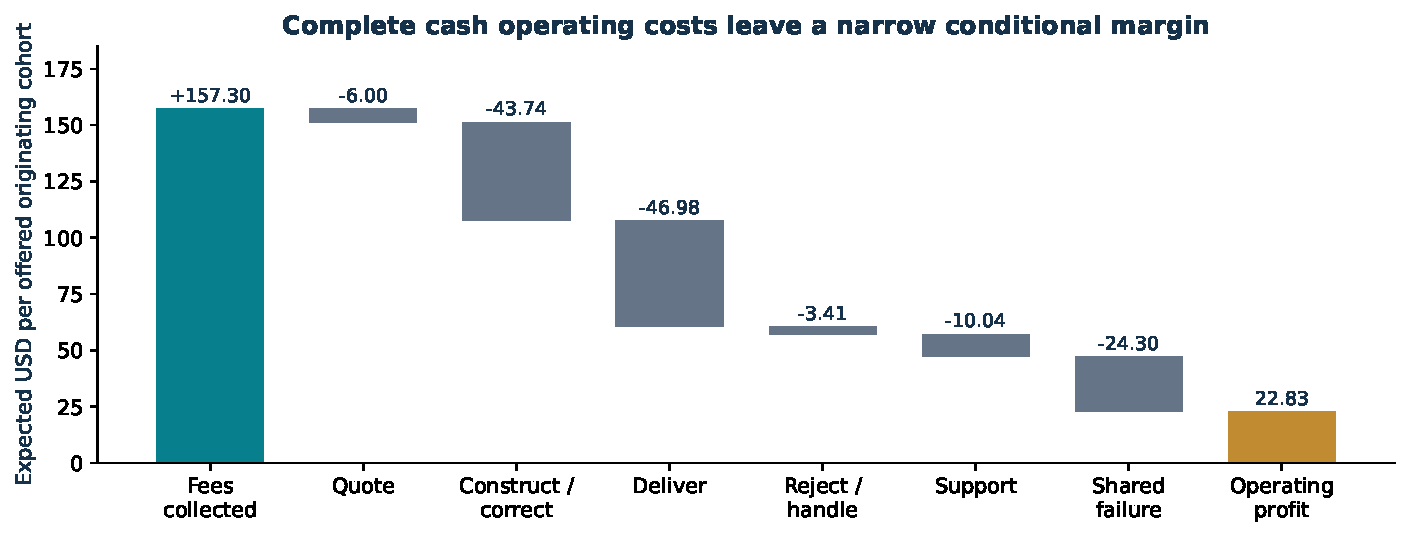
\includegraphics{figures/economics.pdf}
\caption{All modeled paid-job cash costs are charged once. The expected
positive result is small relative to plausible uncertainty in delivery
effort and common failure. Extra retention and R\&D are separate
decisions.}
\end{figure}

The same economic policy was then applied to all 48 fresh cases. It
placed \textbf{zero orders} and collected \textbf{zero modeled service
revenue}. Preliminary quoting/assessment still cost \$346. Counting
those rejected opportunities changes the modeled invitation campaign to
\textbf{−\$323.17} before B/C. The original positive illustration is
preserved, but it does not establish a profitable general enterprise or
a growing frontier of sellable work.

\hypertarget{human-service-reference-and-buyer-value}{%
\subsection{Human-service reference and buyer
value}\label{human-service-reference-and-buyer-value}}

The BLS reports a May 2025 median aerospace-engineer annual wage of
\$134,960. (\protect\hyperlink{ref-bls2026}{US Bureau of Labor
Statistics 2026}) Dividing by an assumed 2,080 hours gives the study's
hourly proxy of \$64.8846. For the same finite decision-support scope,
assumed work of 8--24 hours and burden multipliers of 1.5--2.5 give a
human-production cost scenario of approximately \textbf{\$779--\$3,893}.
Hours, burden and exact scope are estimates; this is not a consulting
quote, flight certification price or proof that buyers would pay that
amount.

The specialized shared-observation arrangement has no verified
human-service market quote. Its primary price/participation test
therefore uses explicit avoided-action-cost and willingness-to-pay
hypotheses. The executable outside option is the supplied
baseline/fallback plan. Free screening is a real-world alternative to
qualify before a trial; it is not a separately priced and executed
choice arm here. A sufficiently equipped conventional expert remains an
equal technical competitor. Human cost, buyer savings and token issuance
are not enterprise revenue.

\hypertarget{liquidity-failure-and-liabilities}{%
\subsection{Liquidity, failure and
liabilities}\label{liquidity-failure-and-liabilities}}

The all-commit, all-accept, all-pay illustration receives \$840: \$600
is acquisition pass-through and \$240 is service revenue. Complete A
cost is \$135, leaving \$105 operating contribution. Seed capital of
\$1,500 ends as \$1,605; after a \$300 provider reserve, \$1,305 is
available. The buyers separately need \$800, \$950 and \$1,100 under the
stated cash timing, including the full fee and fallback reserves of
\$500, \$650 and \$800. Their actual balances are unknown.

An early ledger version reserved only the fee deposit on the buyer side.
Review caught the omitted unpaid balance. The original source/results
are preserved, the full-fee correction has a targeted regression, and
primary expected profit is unchanged. This correction is part of the
result, not an erased preparation error.

\begin{figure}
\centering
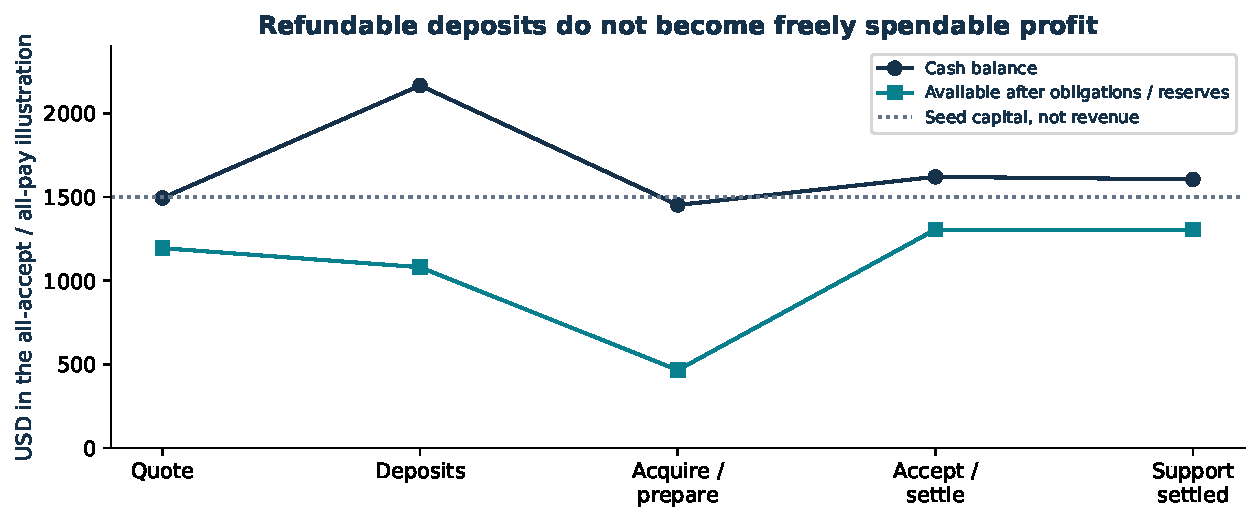
\includegraphics{figures/liquidity.pdf}
\caption{Cash and available funds differ throughout the modeled
successful branch. Refundable deposits, unpaid obligations and reserves
remain visible. These time steps are bookkeeping order, not measured
end-to-end satellite-service latency.}
\end{figure}

For cumulative net cash flow excluding seed \(F_t\), refundable
liability \(L_t\), unpaid obligations \(O_t\) and reserve \(R\),
required seed is

\[
S_{\rm req}=\max\left(0,\max_t\{L_t+O_t+R-F_t\}\right).
\]

The zero-seed stress needs up to \textbf{\$1,050} of financing and is
unexecutable without it, despite positive expected source contribution.
The worst source outcome loses \$750. Raising conditional fee-balance
default to 100\% changes expected contribution to −\$86.27. A postcommit
withdrawal after acquisition leaves \$20 in the explicit
two-pay/one-withdraw branch, while retaining sunk cost and refund
obligations. No default or refund is charged twice.

\hypertarget{transfer-selective-retention-and-the-next-opportunity}{%
\section{Transfer, selective retention and the next
opportunity}\label{transfer-selective-retention-and-the-next-opportunity}}

The retained asset is a small executable compiler plus its scope
contract, packaged as an exact two-file archive. It contains no
protected cases or answers. It records version, license, source
identities, prerequisites and limitations. The artifact is
researcher-constructed and revised through development feedback. It is
not a weight-trained model, a learned sensor probability matrix or
evidence of autonomous scientific invention.

The existing source-qualified integration closure is reused unchanged:
29 vendor/lifecycle/native files within a 34-file bridge/driver closure.
Its controls exercise member access, revocation, stale baseline, rights
refusal, protected material and signed A/B/C accounting. \textbf{29 of
29} conformance controls pass. The conformance driver uses artificial
admission economics; those controls do not admit this capability on
empirical profit evidence. Native scientific scope remains refused
rather than expanded to make the experiment pass.

\hypertarget{a-separate-recipient-actually-executes-the-bytes}{%
\subsection{A separate recipient actually executes the
bytes}\label{a-separate-recipient-actually-executes-the-bytes}}

The recipient was selected by the lowest ID in the unfamiliar withdrawal
category, not by its gain. It contains five latent states, three
remaining operators and eighteen branches, compared with the source
mission's two states and nine branches. The exact retrieved archive runs
in a separate isolated process. Thirteen transfer/process/parity checks
pass, and the independent checker passes 174 comparisons.

\begin{longtable}[]{@{}lr@{}}
\toprule\noalign{}
Fresh recipient quantity & Modeled USD \\
\midrule\noalign{}
\endhead
\bottomrule\noalign{}
\endlastfoot
Baseline action expense & \$236.84 \\
Contingent action expense & \$100.60 \\
Aggregate gross information value & \textbf{\$136.24} \\
Operator 0 information value & \textbf{−\$16.03} \\
Operator 1 information value & \$103.44 \\
Operator 3 information value & \$48.83 \\
\end{longtable}

An aggregate surplus does not demonstrate voluntary participation. The
full-roster offer has an individually losing buyer, and the unchanged
commercial policy declines it. Even the strongest voluntary subset
supports only about \$0.04 of acquisition expense at the fixed \$80 fee;
provider economics are negative there. None of the 25 predeclared
price/acquisition diagnostic cells yields a viable recipient order. The
successor therefore produces a justified stop, with a clear reason and
preserved evidence.

An ordinary directory containing the same compiler and scope contract
yields byte-identical output. This rejects a graph-specific value claim.
The recipient can use the instrument without rebuilding it, but the
study has not measured additional paid effort saved relative to a
competent recipient already holding an equivalent conventional program.

\hypertarget{investment-must-be-reachable-before-assessment}{%
\subsection{Investment must be reachable before
assessment}\label{investment-must-be-reachable-before-assessment}}

With incremental per-use cash saving \(g\), upkeep \(m\), initial B cost
and optional extra C, strictly positive retained value requires

\[
N(g-m)>B+C.
\]

At \(g=0\), the admission rule rejects retention before paying for an
unattainable assessment. At the hypothetical \(g=10\) and \(m=2\),
B=\$180 needs 23 compatible uses; adding optional C=\$240 needs 53.
These are conditional break-even thresholds, not measured savings,
guaranteed demand or admitted Alpha. Obsolescence, unfamiliar scope,
negative transfer and uncertain reuse can only tighten the decision.

\begin{figure}
\centering
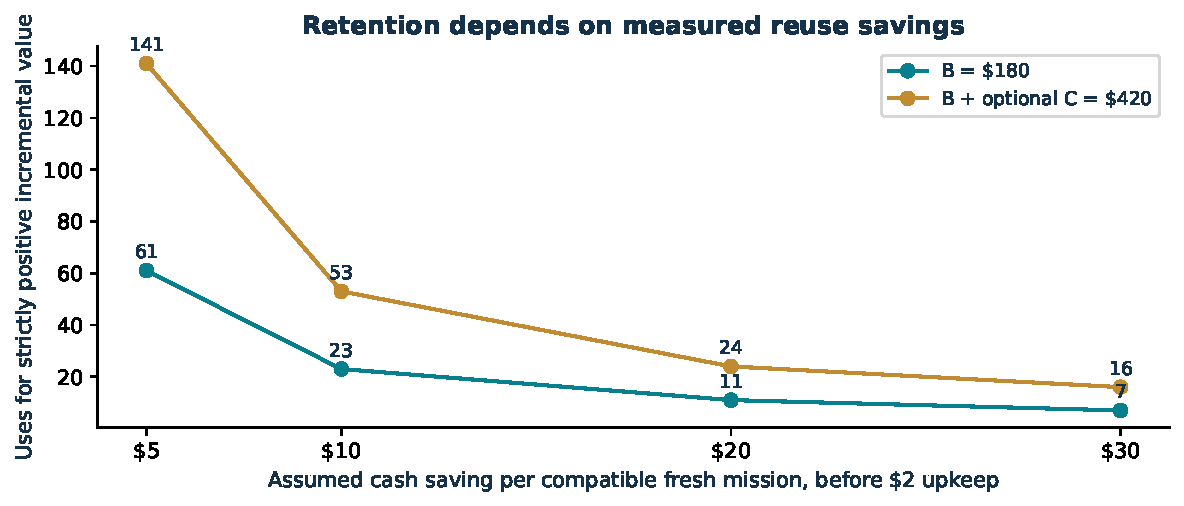
\includegraphics{figures/retention.pdf}
\caption{Reuse must repay additional costs against the recipient's
competent baseline. Incremental commercial savings remain unmeasured, so
commercial admission is on hold. The research artifact remains available
for inspection and reproduction.}
\end{figure}

\hypertarget{frontier-operation-and-prompting-a-proportionate-test-plan}{%
\section{Frontier operation and prompting: a proportionate test
plan}\label{frontier-operation-and-prompting-a-proportionate-test-plan}}

Official documentation retrieved on 27 October 2026 identifies
\texttt{gpt-6-astra} for demanding reasoning and research and
\texttt{gpt-6.1-terra} for visual/computer-use work. Both expose tool
use; project access and actual API entitlement were not established.
Local presence checks found an installed SDK but no configured API key.
ChatGPT subscription access does not establish API billing or a
reproducible provider trial. (\protect\hyperlink{ref-astra}{OpenAI
2026b}, \protect\hyperlink{ref-terra}{2026c})

\begin{longtable}[]{@{}
  >{\raggedright\arraybackslash}p{(\columnwidth - 2\tabcolsep) * \real{0.5000}}
  >{\raggedleft\arraybackslash}p{(\columnwidth - 2\tabcolsep) * \real{0.5000}}@{}}
\toprule\noalign{}
\begin{minipage}[b]{\linewidth}\raggedright
Model
\end{minipage} & \begin{minipage}[b]{\linewidth}\raggedleft
Standard input / output / cached input, USD per million tokens
\end{minipage} \\
\midrule\noalign{}
\endhead
\bottomrule\noalign{}
\endlastfoot
\texttt{gpt-6-astra} & \$10 / \$50 / \$1 \\
\texttt{gpt-6.1-terra} & \$1 / \$5 / \$0.05 \\
\texttt{gpt-6.1-sol} & \$2 / \$10 / \$0.10 \\
\end{longtable}

These are tariffs, not observed study bills. The primary model uses
short contexts without a cache benefit. Above 272,000 input tokens,
Astra/Terra input/cache rates double and output rates rise by 1.5; cache
writes and tool environments can cost extra.
(\protect\hyperlink{ref-pricing}{OpenAI 2026a},
\protect\hyperlink{ref-astra}{2026b},
\protect\hyperlink{ref-terra}{2026c}) The frozen assumed
30,000-input/10,000-output Astra workload costs \$0.80 before additional
tools, already included in A. Token counts, semantic accuracy and
latency remain hypotheses.

The versioned reusable expert method is: capture original purpose and
outside options; validate source meaning and units; enumerate adverse
and missing-result branches; construct the minimal plan; independently
check it; reconcile participation and funding; deliver or refuse with an
auditable reason. The supplied prompt cards, authored after this
software confirmation for the next matched trial, give U the same
model/tool opportunities and usable context, E this checklist, and E+
the actual artifact. They were not the protocol behind the recorded 48
cases. Prompt sophistication does not set acceptance probabilities.

Primary simulated semantic acceptance is \(q_U=q_E=q_{E+}=0.90\). A
separate assumption grid includes equality, worse outcomes, positive
gains, resource multipliers and retry costs. At matched resources it
compares acceptance; at matched accepted quality it compares expected
cost per accepted outcome. It does not treat a larger token budget as
Operational Alpha.

For contracted price \(P\), fee deposit fraction \(f\), default
probability \(d\) on the remaining balance, effective per-package
acceptance probability \(Q_k=(1-c)q_k\) and complete expected
attempted-job cost \(a_k\), the collectible-price factor is
\(h=1-(1-f)d\). For an equal fixed roster, \(Q_k\) is the expected
accepted-fee fraction, not the probability that every package passes:

\[
\pi_k=Q_kPh-a_k,\qquad
\Delta Q_{E-U}>\frac{a_E-a_U}{Ph}.
\]

The primary deposit/default assumptions give \(h=0.979\). For a fixed
three-package illustration, \$20 of extra expert cost on \$240 of
contracted fees requires \textbf{8.5121 percentage points} of additional
effective per-package acceptance. Expressed as conditional semantic
acceptance with common failure fixed at 5\%, the required improvement is
\textbf{8.9601 points}. An extra \$30 requires 13.4401 conditional
points, exceeding the remaining room from a 90\% baseline. This marginal
illustration holds the roster and other costs fixed; the full event tree
separately models individual participation and withdrawals. The
analytics correction and its prior version are preserved. The next
matched trial should measure these quantities; this deterministic
software experiment supplies no empirical frontier-model gain.

\hypertarget{what-the-simulation-usefully-establishes}{%
\section{What the simulation usefully
establishes}\label{what-the-simulation-usefully-establishes}}

The conditional source example works only when information benefit,
voluntary participation, supplier price, package effort and funding
jointly fit. At the frozen \$80 fee, the strongest source coalition's
acquisition ceiling is \textbf{\$706.34}. At that exact boundary, the
event tree still has positive expected contribution of \$19.08. The
ceiling is an inverse-price diagnostic derived after confirmation, not
an observed supplier quote or a new primary result.

\begin{figure}
\centering
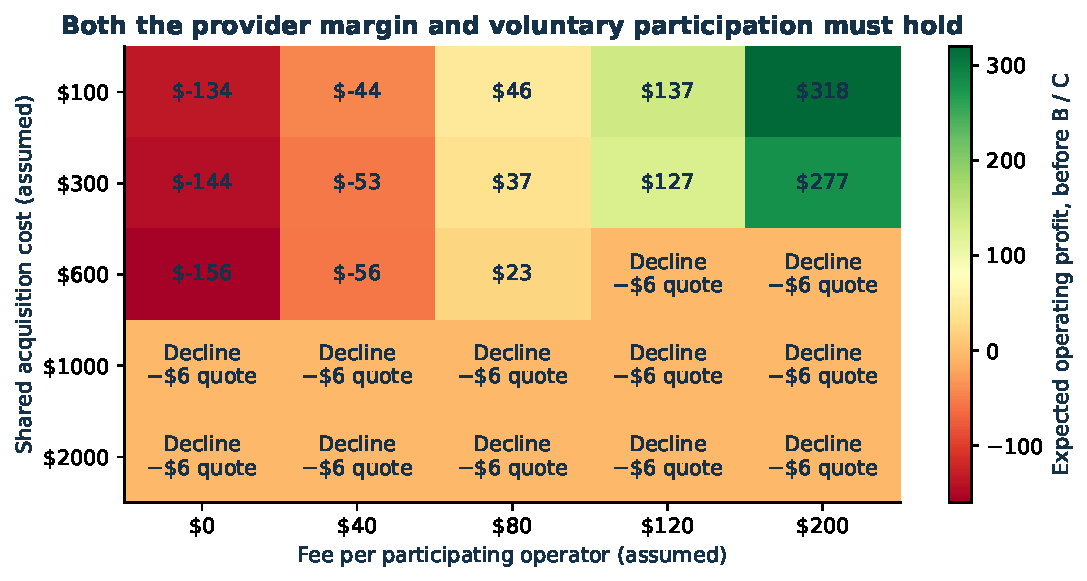
\includegraphics{figures/feasibility.pdf}
\caption{The source offer has a bounded commercial region. Larger fees
can eliminate participation; inexpensive acquisition does not make a
zero-fee service profitable. All cells are exact arithmetic under
declared assumptions.}
\end{figure}

For equal shares, a voluntary subset \(S\) has acquisition ceiling

\[
K_{\max}(S)=|S|\left[q\left(\min_{i\in S}V_i-p\right)-\frac{a}{1-c}\right].
\]

This gives the smallest useful next question: can an appropriate
provider deliver timely, actionable information below the relevant
ceiling, and do actual operators agree with the modeled values and
obligations? More simulated draws cannot answer that question. The
current fresh cohort's zero orders and negative total invitation
contribution make broad commercialization or compulsory training
unsupported.

There are two kinds of uncertainty. Within a specified world, the exact
event tree determines expected collections and losses. Across worlds,
the probabilities, effort, buyer values, sensor behavior and contractual
terms are uncertain assumptions. The latter dominate the result. No
narrow numerical confidence band can convert them into empirical demand
or physical assurance.

\hypertarget{practical-operating-blueprint}{%
\section{Practical operating
blueprint}\label{practical-operating-blueprint}}

The general operating path extends the existing system without a
competing registry:

\begin{enumerate}
\def\labelenumi{\arabic{enumi}.}
\tightlist
\item
  \textbf{Discover and qualify the need.} Record beneficiary, original
  useful outcome, outside options, overlap with active work and the
  cheapest falsifier. Reject generic novelty claims when a conventional
  method already supplies the claimed capability.
\item
  \textbf{Freeze the commercial and technical contract.} Record quality,
  deadline, customer effort, permissions, price and failure handling.
  Separate supplied assumptions from observed evidence and preserve a
  source identity for each.
\item
  \textbf{Construct the smallest instrument.} Charge learning necessary
  for the paid outcome to A. Keep every adverse-result and timeout
  branch. Use an independent conventional implementation with equal
  information and rights.
\item
  \textbf{Gate each proposed offer.} Check mission-specific semantics,
  each participant's utility, original fallback resources, funding
  prefixes and all obligations. Refuse zero-value information and
  unaffordable or incompatible offers.
\item
  \textbf{Accept and account.} Bind artifact, acceptance, source,
  permissions and cost records. Separate pass-through funds from earned
  fees; retain refunds, defaults and support. Treat actual missing
  billing as unknown.
\item
  \textbf{Retain selectively.} Assess incremental value against the
  recipient's competent baseline before paying further admission cost.
  Rights-clear and version the actual executable asset. Withhold
  protected evaluation material and secrets.
\item
  \textbf{Transfer and revalidate.} Reuse stable identity and scope
  qualifications only when unchanged. Recheck the new mission's inputs,
  outputs and meaning. Grant authority through its existing separate
  process. Preserve Jobs validator and settlement boundaries.
\item
  \textbf{Choose the next opportunity or stop.} A correct refusal is
  useful operating information. It is not a sale, new
  productive-frontier crossing or earned reinvestment capital.
\end{enumerate}

The public research artifact is inspectable, while the fixture lifecycle
exercises sharing among authorized \texttt{*.agent.agi.eth} identities.
Those fixture checks do not establish live ENS authentication or
production scope. The source-qualified journal and cost ledger remain
authoritative for their existing boundaries. No token minting, wallet
action or \texttt{\$AGIALPHA} utility is counted as operating profit.

\hypertarget{next-experiment-and-decision-rules}{%
\section{Next experiment and decision
rules}\label{next-experiment-and-decision-rules}}

The next live step is deliberately small: one observation provider and
two or three operators supply a retrospective, permission-cleared event
with an explicit shared-information opportunity. Obtain a scoped
provider quote, the operators' existing alternatives and the action/cash
obligations they actually retain. No observation should be purchased
merely to validate this paper's example.

Run a shadow exercise first. Use an established conjunction-analysis
process for domain inputs; the new instrument handles conditional
packaging and accounting. Compare a competent conventional expert and
the retained workflow with identical evidence, model access, budgets and
permission to propose alternatives. Freeze the procedure, acceptance
terms and budgets before revealing the held-out observation and outcome.
Measure preparation, tokens/tools, failed attempts, correction, latency,
customer effort and acceptance. Include one adverse/missing-result case
and a buyer withdrawal. Record actual supplier and buyer terms before
evaluating the outcome.

Before an authorized pilot, require original-purpose qualification,
willing participants, a favorable complete expected contribution under
their agreed terms, and sufficient funding for every cash prefix. After
delivery, assess actual acceptance, collections and realized
contribution separately. Test retention only if measured incremental
recipient savings support reachable repayment before expected
obsolescence. The source illustration's \$706.34 acquisition ceiling,
\$22.83 unpriced-cost tolerance and reuse thresholds provide falsifiable
starting conditions, not approval to spend.

The current decision is to preserve the reusable research instrument,
hold commercial admission, and seek the smallest price/value evidence
capable of changing that decision. This completes the experimental cycle
while leaving an explicit next question.

\hypertarget{reproducibility-provenance-and-remaining-limits}{%
\section{Reproducibility, provenance and remaining
limits}\label{reproducibility-provenance-and-remaining-limits}}

The study is additive to main source
\texttt{47c17f6aca6b1bb8779dd3e47d5ba5f8af3329f4}; it retains
predecessor research \texttt{231834269599d85e49cfe1ca9917a1a874522d44}
and native closure pins. Earlier thermal, numerical, manufacturing,
ecological and operational studies remain unchanged. Source versions and
ownership were inspected through issue 4850 before selecting this
distinct lane.

The complete package includes source inputs, all 48 cases, candidate and
reference outputs, process logs, preserved development
failures/corrections, exact cost assumptions, the event tree, native
transfer/accounting evidence, source hashes, this LaTeX project, an
executive brief, an evidence companion and an English/French
demonstration. The browser edition reproduces the manuscript. Canonical
publication remains subject to the existing review and owner-controlled
release process; a local reader or draft source link is not a deployed
Pages edition.

Reproduction uses Python 3.11--3.13 for the study and the recorded
Node/Pydantic/cryptography environment for the inherited integration.
Core inference and finite economic enumeration require only the standard
library. Scientific figure/document construction adds Matplotlib and the
available LaTeX/Pandoc toolchain. The README provides commands with
fresh output directories so original evidence is not overwritten.

The implementation was designed, coded, executed and written with
ChatGPT assistance at the author's request. Separate same-session agents
handled discovery, calibration, reference evaluation and integration.
Their separation improves review but is not external peer review. The
stated author attribution does not imply that the author personally
conducted every execution or has approved a final public deployment.

The study does not measure physical collision safety, sensor-model
calibration, customer demand, enforceable agreements, live settlement,
complete realized research cost, independent specialist training or
sustained compounding. The exact conventional and ordinary-library ties
are retained. The positive source example and negative fresh economic
cohort are equally part of the result. What remains is a working
instrument, a reproducible conditional argument and a more selective
path to the next useful experiment.

\hypertarget{bibliography}{%
\section*{References}\label{bibliography}}
\addcontentsline{toc}{section}{References}

\hypertarget{refs}{}
\begin{CSLReferences}{1}{0}
\leavevmode\vadjust pre{\hypertarget{ref-esa2021}{}}%
European Space Agency. 2021. {``Blockchain Ecosystem for an Autonomous
Consensus Mechanism of Federated Satellite Networks.''}
\url{https://ideas.esa.int/core/servlet/hype/IMT?documentId=2d929ce255874896a6a09107ed58060f\&documentTableId=7295537402235904412\&templateName=\&userAction=Browse}.

\leavevmode\vadjust pre{\hypertarget{ref-phisat}{}}%
---------. 2023. {``PhiSat-2 Mission Overview for the OrbitalAI
Challenge.''}
\url{https://challenges.philab.esa.int/wp-content/uploads/2023/02/Phisat-2_Mission_Overview_Web.pdf}.

\leavevmode\vadjust pre{\hypertarget{ref-coldchain}{}}%
FAO and UNEP. 2022. {``Amid Food and Climate Crises, Investing in
Sustainable Food Cold Chains Crucial.''}
\url{https://www.fao.org/newsroom/detail/amid-food-and-climate-crises-investing-in-sustainable-food-cold-chains-crucial/en}.

\leavevmode\vadjust pre{\hypertarget{ref-economy}{}}%
MONTREAL.AI. 2026a. {``Invent the Economy: Transformational Intelligence
for Creating Viable Markets.''}
\url{https://github.com/MontrealAI/AGI-Alpha-Agent-v0/blob/231834269599d85e49cfe1ca9917a1a874522d44/docs/Invent_the_Economy.tex}.

\leavevmode\vadjust pre{\hypertarget{ref-coordination}{}}%
---------. 2026b. {``SUCCESSOR Omega Public Integration Coordination,
Issue 4850.''}
\url{https://github.com/MontrealAI/AGI-Alpha-Agent-v0/issues/4850\#issuecomment-6448140155}.

\leavevmode\vadjust pre{\hypertarget{ref-harness}{}}%
---------. 2026c. {``Transformational Autonomous Enterprises: SUCCESSOR
Omega Harness.''}
\url{https://github.com/MontrealAI/AGI-Alpha-Agent-v0/blob/231834269599d85e49cfe1ca9917a1a874522d44/docs/papers/transformational-autonomous-enterprises-v1.tex}.

\leavevmode\vadjust pre{\hypertarget{ref-ti}{}}%
---------. 2026d. {``Transformational Intelligence: Learning to Change
the Game.''}
\url{https://github.com/MontrealAI/AGI-Alpha-Agent-v0/blob/231834269599d85e49cfe1ca9917a1a874522d44/docs/Transformational_Intelligence.tex}.

\leavevmode\vadjust pre{\hypertarget{ref-nasa2026}{}}%
NASA Office of the Chief Engineer. 2026. {``Spacecraft Conjunction
Assessment and Collision Avoidance Best Practices Handbook: Volume 1.''}
\url{https://nodis3.gsfc.nasa.gov/OCE_docs/OCE_51.pdf}.

\leavevmode\vadjust pre{\hypertarget{ref-pricing}{}}%
OpenAI. 2026a. {``API Pricing.''}
\url{https://developers.openai.com/api/docs/pricing}.

\leavevmode\vadjust pre{\hypertarget{ref-astra}{}}%
---------. 2026b. {``GPT-6 Astra Model.''}
\url{https://developers.openai.com/api/docs/models/gpt-6-astra}.

\leavevmode\vadjust pre{\hypertarget{ref-terra}{}}%
---------. 2026c. {``GPT-6.1 Terra Model.''}
\url{https://developers.openai.com/api/docs/models/gpt-6.1-terra}.

\leavevmode\vadjust pre{\hypertarget{ref-uriot2020}{}}%
Uriot, Thomas, Dario Izzo, Luís F. Simões, Rasit Abay, Nils Einecke,
Sven Rebhan, Jose Martinez-Heras, Francesca Letizia, Jan Siminski, and
Klaus Merz. 2020. {``Spacecraft Collision Avoidance Challenge: Design
and Results of a Machine Learning Competition.''}
\emph{arXiv:2008.03069}. \url{https://arxiv.org/abs/2008.03069}.

\leavevmode\vadjust pre{\hypertarget{ref-bls2026}{}}%
US Bureau of Labor Statistics. 2026. {``Aerospace Engineers:
Occupational Outlook Handbook.''}
\url{https://www.bls.gov/ooh/architecture-and-engineering/aerospace-engineers.htm}.

\leavevmode\vadjust pre{\hypertarget{ref-epa}{}}%
US Environmental Protection Agency. 2026. {``Tackling Emerging
Contaminants.''}
\url{https://www.epa.gov/water-infrastructure/tackling-emerging-contaminants-tec}.

\end{CSLReferences}
\end{document}
